\chapter {Các công trình nghiên cứu liên quan}

\section{Pulpissimo}

\subsection{Tổng quan}
Pulpissimo (PULP Independent Single-stream Shared-memory Integrated Subsystem for MOtion control) 
là một hệ thống vi điều khiển (Microcontroller System) tiên tiến dựa trên kiến trúc RISC-V 32-bit, 
được phát triển bởi nhóm nghiên cứu PULP (Parallel Ultra Low Power) thuộc ETH Zürich và Đại học Bologna.

Mục tiêu thiết kế của Pulpissimo là cung cấp một nền tảng phần cứng linh hoạt, tiết kiệm năng lượng 
nhưng vẫn đảm bảo hiệu năng tính toán cao cho các ứng dụng IoT và Edge AI yêu cầu băng thông lớn. 
Khác với các vi điều khiển truyền thống, Pulpissimo không chỉ là một lõi CPU đơn lẻ mà là một hệ thống 
SoC (System-on-Chip) hoàn chỉnh với kiến trúc bộ nhớ và ngoại vi thông minh  \cite{pulpissimo}.

\begin{figure}[!h]
    \centering
    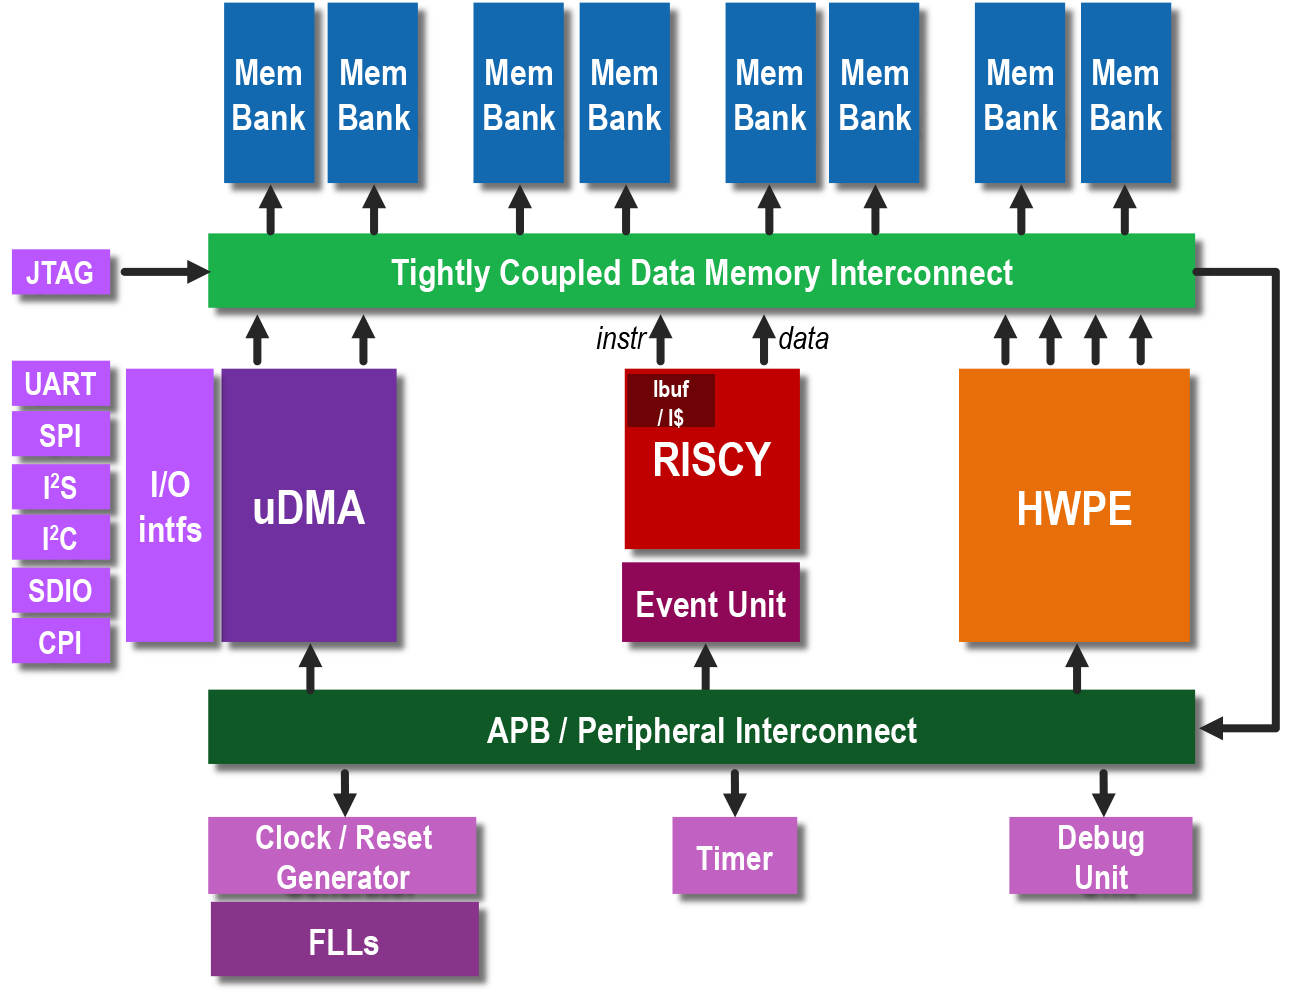
\includegraphics[width=0.7\linewidth]{images/congtrinhlienquan/pulpissimo_archi.png}
    \caption{Kiến trúc Pulpissimo}
    \label{fig:pulpissimo_archi}
\end{figure}

\subsection{Các đặc điểm kỹ thuật nổi bật}
PULPissimo bao gồm các thành phần chính sau:
\begin{itemize}
    \item Bộ xử lý chính: Hoặc bộ xử lý RI5CY hoặc bộ xử lý Ibex
    \item Hệ thống con uDMA: Hệ thống con đầu vào/đầu ra tự động để quản lý thiết bị ngoại vi hiệu quả
    \item Hệ thống con bộ nhớ: Bao gồm ROM khởi động và bộ nhớ L2
    \item Hệ thống sự kiện và ngắt: Bộ điều khiển ngắt đơn giản để quản lý các sự kiện hệ thống
    \item Thiết bị ngoại vi: Bao gồm SPI, I2S, giao diện camera, I2C, UART, Hyperbus và GPIO
    \item Bộ xử lý phần cứng (HWPE): Hỗ trợ các bộ tăng tốc phần cứng tùy chỉnh
\end{itemize}
\subsubsection{Lõi xử lý RI5CY/CV32E40P}
Trung tâm của Pulpissimo là nhân xử lý RI5CY (hiện nay được chuẩn hóa thành CV32E40P bởi OpenHW Group). 
Đây là một hiện thực hóa (implementation) của RISC-V với đường ống 4 tầng, được tối ưu hóa đặc biệt cho 
xử lý tín hiệu số (DSP).
Điểm đặc biệt của nhân này là việc hỗ trợ các mở rộng tập lệnh không tiêu chuẩn (Non-standard Extensions) 
giúp tăng tốc đáng kể các thuật toán AI:
\begin{itemize}
    \item \textbf{Hardware Loops:} Cho phép thực hiện các vòng lặp mà không tốn chu kỳ máy cho 
    việc kiểm tra điều kiện và rẽ nhánh.
    \item \textbf{SIMD (Single Instruction Multiple Data):} Hỗ trợ tính toán song song trên các 
    vector nhỏ (ví dụ: thực hiện 2 phép cộng 16-bit hoặc 4 phép cộng 8-bit trong 1 chu kỳ). 
    Đây là tính năng then chốt để xử lý dữ liệu lượng tử hóa (Quantized Data) trong mạng nơ-ron.
    \item \textbf{Bit Manipulation:} Các lệnh thao tác bit giúp tối ưu hóa việc đóng gói và giải nén 
    dữ liệu trọng số.
\end{itemize}

\subsubsection{Hệ thống bộ nhớ và uDMA}
Để giải quyết bài toán "nghẽn cổ chai" dữ liệu, Pulpissimo sử dụng bộ điều khiển truy cập bộ nhớ 
trực tiếp thông minh (micro-DMA hay uDMA). uDMA cho phép truyền dữ liệu trực tiếp từ các ngoại 
vi tốc độ cao (như Camera Interface, SPI) vào bộ nhớ nội (L2 Memory) mà không cần sự can thiệp 
của CPU. Cơ chế này giúp CPU có thể chuyển sang trạng thái ngủ (Sleep Mode) trong khi dữ liệu đang 
được thu thập, giúp tiết kiệm năng lượng tối đa .

\newpage
\section{Mạng nơ-ron Nhị phân (BNN)}

Trong nỗ lực giảm thiểu tài nguyên phần cứng cho các thiết bị biên, BNN nổi lên như một hướng 
nghiên cứu đột phá, đặc biệt phù hợp với cấu trúc của FPGA. Công trình nền tảng của Courbariaux 
và cộng sự \cite{bnn_courbariaux} đã chứng minh khả năng huấn luyện các mạng nơ-ron 
sâu với trọng số và tín hiệu kích hoạt bị ràng buộc ở hai mức giá trị.

\subsection{Cơ sở toán học và Nguyên lý hoạt động}

\subsubsection{Hàm nhị phân hóa (Binarization Function)}
Khác với các mạng CNN truyền thống sử dụng số thực 32-bit (FP32), BNN ép buộc các trọng số (Weights) 
và giá trị kích hoạt (Activations) về miền giá trị $\{+1, -1\}$. Courbariaux đề xuất hai phương pháp 
nhị phân hóa:
\begin{itemize}
    \item \textbf{Nhị phân hóa tất định (Deterministic Binarization):} Sử dụng hàm dấu (Sign function):
    \begin{equation}
        x^b = \text{Sign}(x) = \begin{cases} +1 & \text{if } x \geq 0 \\ -1 & \text{if } x < 0 \end{cases}
    \end{equation}
    Đây là phương pháp thường được sử dụng trong giai đoạn suy luận (Inference) trên phần cứng.
    \item \textbf{Nhị phân hóa ngẫu nhiên (Stochastic Binarization):} Sử dụng xác suất dựa trên 
    hàm sigmoid, thường dùng trong quá trình huấn luyện để tránh bị kẹt ở cực trị cục bộ, 
    tuy nhiên ít được áp dụng khi triển khai phần cứng do chi phí tính toán cao.
\end{itemize}

\subsubsection{Chiến lược huấn luyện với Straight-Through Estimator (STE)}
Thách thức lớn nhất khi huấn luyện BNN là hàm $\text{Sign}(x)$ không khả vi 
(đạo hàm bằng 0 ở hầu hết mọi nơi), khiến thuật toán lan truyền ngược (Backpropagation) không thể 
cập nhật trọng số.
Để giải quyết vấn đề này, Courbariaux áp dụng kỹ thuật \textbf{Straight-Through Estimator (STE)}. 
Trong quá trình lan truyền ngược, gradient được truyền xuyên qua hàm dấu mà không bị biến đổi 
(hoặc chỉ bị cắt bởi hàm Hard Tanh), coi như hàm dấu là hàm đồng nhất (Identity function) 
trong một khoảng nhất định:
\begin{equation}
    g_x \approx g_{x^b} \cdot \mathbf{1}_{|x| \le 1}
\end{equation}
Nhờ đó, mạng BNN có thể được huấn luyện "End-to-end" tương tự như các mạng CNN thông thường.

\subsection{Kiến trúc phần cứng trên FPGA}

Lợi thế cốt lõi của BNN nằm ở việc thay thế các phép toán đại số tuyến tính tốn kém bằng các phép toán 
logic bit-wise:

\begin{itemize}
    \item \textbf{Thay thế bộ nhân (Multiplier-less):} Phép nhân giữa một giá trị nhị phân 
    kích hoạt $a \in \{+1, -1\}$ và trọng số $w \in \{+1, -1\}$ có thể được mô hình hóa chính 
    xác bằng phép toán cổng \textbf{XNOR}:
    \begin{equation}
        a \cdot w \Leftrightarrow \neg(a \oplus w)
    \end{equation}
    Trên FPGA, một cổng XNOR tiêu tốn tài nguyên LUT không đáng kể so với một khối DSP48E2 dùng cho 
    phép nhân số thực.
    
    \item \textbf{Thay thế phép cộng (Accumulation):} Phép tích chập (Convolution) bao gồm việc tính 
    tổng các tích số. Trong BNN, thao tác này trở thành việc đếm số lượng bit 1 trong vector 
    kết quả XNOR, gọi là phép \textbf{Popcount} (Population Count). 
    \begin{equation}
        \mathbf{a} \cdot \mathbf{w} \approx 2 \cdot \text{popcount}(\text{xnor}(\mathbf{a}, 
        \mathbf{w})) - N
    \end{equation}
    (Với $N$ là độ dài vector).
\end{itemize}

\subsection{Hiệu quả tài nguyên và Giới hạn}
Theo kết quả thực nghiệm từ bài báo gốc, việc sử dụng BNN giúp giảm kích thước bộ nhớ xuống 
\textbf{32 lần} so với FP32, cho phép toàn bộ mô hình (hoặc các lớp lớn) nằm gọn trong bộ nhớ nội 
(Block RAM/UltraRAM) của FPGA. Điều này loại bỏ nút thắt cổ chai về băng thông bộ nhớ ngoài 
(Von Neumann bottleneck), giúp tăng tốc độ xử lý lên đáng kể.

\begin{figure}[!h]
    \centering
    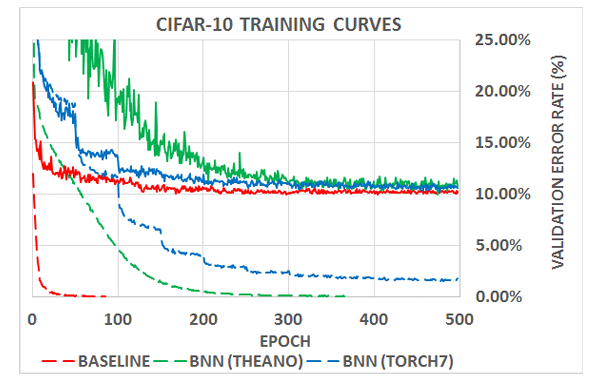
\includegraphics[width=0.8\linewidth]{images//congtrinhlienquan/bnn.png}
    \caption{Đường cong huấn luyện của mạng ConvNet trên tập dữ liệu CIFAR-10 tùy thuộc vào phương pháp.}
    \label{fig:placeholder}
\end{figure}

Tuy nhiên, BNN cũng bộc lộ hạn chế về độ chính xác (Accuracy Drop), đặc biệt với các bộ dữ liệu 
phức tạp như ImageNet. Do đó, trong đồ án này, chúng tôi tham khảo nguyên lý tối ưu phần cứng 
của BNN nhưng lựa chọn giải pháp \textbf{Lượng tử hóa 8-bit (INT8)} để đạt được sự cân bằng tối ưu 
giữa độ chính xác và hiệu năng trên nền tảng Kria KV260. Do đó, trong khuôn khổ đồ án này, 
nhóm nghiên cứu lựa chọn giải pháp lượng tử hóa điểm tĩnh (Fixed-point Quantization) 8-bit hoặc 16-bit 
để đảm bảo sự cân bằng tốt hơn giữa độ chính xác nhận dạng và hiệu năng phần cứng.


%=================================================================================
%=
%=================================================================================
\section{MobileNet}
\label{sec:mobilenet}

MobileNet là lớp các mô hình hiệu quả được Google giới thiệu nhằm phục vụ các ứng dụng thị giác máy tính 
trên thiết bị di động và nhúng. Kiến trúc này dựa trên luồng xử lý tinh gọn, sử dụng tích chập tách biệt 
theo chiều sâu (depthwise separable convolutions) để xây dựng các mạng nơ-ron sâu 
nhưng nhẹ \cite{mobilenet_v1}.

\subsection{Tích chập Tách biệt theo Chiều sâu (Depthwise Separable Convolution)}
Cốt lõi của MobileNet là thay thế cấu trúc tích chập tiêu chuẩn bằng tích chập tách biệt. 
Một lớp tích chập tiêu chuẩn lọc và kết hợp các đặc trưng đầu vào thành tập hợp đầu ra mới 
trong một bước duy nhất. Ngược lại, tích chập tách biệt chia quá trình này thành 
hai lớp riêng biệt:
\begin{enumerate}
    \item \textbf{Depthwise Convolution:} Áp dụng một bộ lọc duy nhất cho mỗi kênh đầu vào 
    để lọc đặc trưng.
    \item \textbf{Pointwise Convolution:} Sử dụng tích chập $1 \times 1$ để tổ hợp tuyến 
    tính các đầu ra từ lớp depthwise.
\end{enumerate}

Xét một lớp tích chập với đầu vào kích thước $D_F \times D_F \times M$ và đầu ra $D_F 
\times D_F \times N$, sử dụng kernel $D_K \times D_K$. 
Chi phí tính toán của tích chập tiêu chuẩn là:
\begin{equation}
    C_{std} = D_K \cdot D_K \cdot M \cdot N \cdot D_F \cdot D_F
\end{equation}

Trong khi đó, chi phí của tích chập tách biệt theo chiều sâu là tổng của hai bước 
(depthwise và pointwise):
\begin{equation}
    C_{sep} = D_K \cdot D_K \cdot M \cdot D_F \cdot D_F + M \cdot N \cdot D_F \cdot D_F
\end{equation}

Tỷ lệ giảm khối lượng tính toán đạt được là:
\begin{equation}
    \frac{C_{sep}}{C_{std}} = \frac{1}{N} + \frac{1}{D_K^2}
\end{equation}
Với MobileNet sử dụng kernel $3 \times 3$, kiến trúc này giúp giảm khối lượng tính toán 
từ 8 đến 9 lần so 
với tích chập truyền thống với mức giảm độ chính xác không đáng kể.

\begin{figure}[!h]
    \centering
    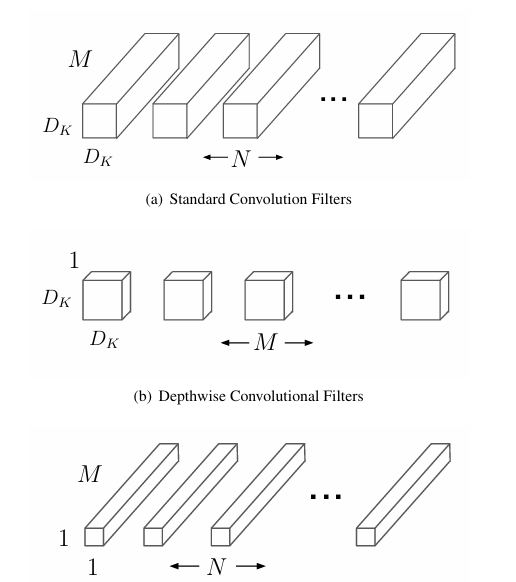
\includegraphics[width=0.7\linewidth]{images/congtrinhlienquan/mobile.png}
    \caption{Kiến trúc của MobileNet với các lớp depthwise và pointwise.}
    \label{fig:mobilenet}
\end{figure}

\subsection{Kiến trúc và Tham số Tinh chỉnh (Hyperparameters)}
\subsubsection{Cấu trúc mạng}
MobileNet bao gồm 28 lớp nếu tính riêng biệt các lớp depthwise và pointwise. Một điểm đặc biệt trong 
thiết kế là 95\% thời gian tính toán của mạng tập trung vào các lớp tích chập $1 \times 1$ (Pointwise). 
Điều này cực kỳ có lợi cho phần cứng FPGA vì tích chập $1 \times 1$ không yêu cầu sắp xếp lại 
bộ nhớ (im2col) và có thể được hiện thực hóa trực tiếp bằng các thuật toán nhân ma trận (GEMM) 
được tối ưu hóa cao.

Tất cả các lớp trong MobileNet đều được theo sau bởi chuẩn hóa theo lô (Batch Normalization) 
và hàm kích hoạt phi tuyến ReLU, ngoại trừ lớp kết nối đầy đủ cuối cùng đưa vào Softmax.

\begin{figure}[!h]
    \centering
    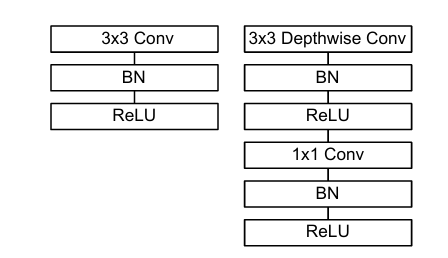
\includegraphics[width=0.8\linewidth]{images/congtrinhlienquan/mobilenet_arch.png}
    \caption{Cấu trúc chi tiết của MobileNetV1}
    \label{fig:mobilenet_archi}
\end{figure}

\newpage
\subsubsection{Các bộ nhân độ rộng và độ phân giải}
Để tùy biến mô hình cho các ràng buộc tài nguyên cụ thể, MobileNet giới thiệu hai tham số siêu hình 
đơn giản:

\begin{itemize}
    \item \textbf{Width Multiplier ($\alpha$):} Có vai trò làm "mỏng" mạng một cách 
    đồng nhất tại mỗi lớp. 
    Với một hệ số $\alpha \in (0, 1]$, số lượng kênh đầu vào $M$ trở thành $\alpha M$ 
    và đầu ra $N$ trở thành $\alpha N$. Chi phí tính toán và số lượng tham số giảm 
    theo hàm bậc hai, xấp xỉ $\alpha^2$[cite: 172].
    \item \textbf{Resolution Multiplier ($\rho$):} Được áp dụng lên hình ảnh đầu vào, 
    làm giảm biểu diễn nội tại của mọi lớp tiếp theo. Hệ số $\rho \in (0, 1]$ giúp giảm 
    chi phí tính toán theo tỷ lệ $\rho^2$.
\end{itemize}

\subsection{Hiệu quả Thực nghiệm}
Các thử nghiệm trên tập dữ liệu ImageNet cho thấy MobileNet đạt hiệu quả vượt trội so với 
các mô hình phổ biến khác.
\begin{itemize}
    \item So với \textbf{VGG16}: MobileNet đạt độ chính xác gần tương đương nhưng có kích 
    thước nhỏ hơn 32 lần và khối lượng tính toán ít hơn 27 lần.
    \item So với \textbf{GoogleNet}: MobileNet chính xác hơn, nhỏ hơn và tính toán ít hơn 2.5 lần.
    \item Khả năng ứng dụng rộng rãi: Ngoài phân loại ảnh, MobileNet còn chứng minh hiệu 
    quả cao trong các tác vụ phát hiện vật thể (Object Detection), phân loại chi tiết 
    (Fine-grain classification), và định vị địa lý quy mô lớn.
\end{itemize}


%=================================================================================
%=
%=================================================================================

\section{Lượng tử hóa và Huấn luyện mạng nơ-ron (Quantization \& Training)}
\label{sec:quantization_theory}

Trong các hệ thống học sâu truyền thống, việc huấn luyện và suy luận thường được 
thực hiện trên định dạng số thực dấu phẩy động 32-bit (Float32) để đảm bảo độ chính xác cao nhất. Tuy nhiên, trên các thiết bị biên (Edge Devices) với tài nguyên hạn chế như FPGA hay vi xử lý nhúng RISC-V, các phép toán số thực tiêu tốn quá nhiều tài nguyên phần cứng và năng lượng.

Để giải quyết vấn đề này, đồ án áp dụng phương pháp lượng tử hóa số nguyên 
được đề xuất bởi \textit{Jacob et al.} (Google) trong công trình 
\textit{"Quantization and Training of Neural Networks for Efficient 
Integer-Arithmetic-Only Inference"} \cite{jacob2018quantization}.

\begin{figure}[!h]
    \centering
    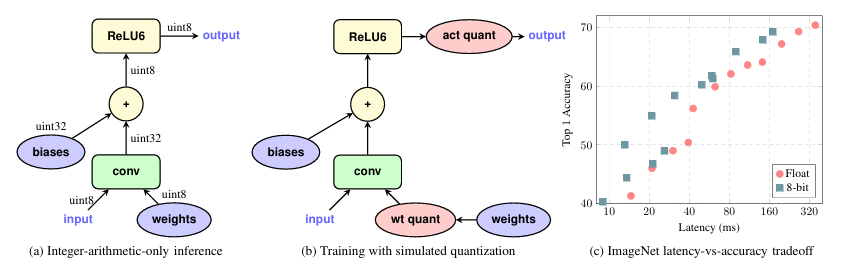
\includegraphics[width=1\linewidth]{images/congtrinhlienquan/quanti.png}
    \caption{Quy trình lượng tử hóa và huấn luyện mạng nơ-ron theo Jacob et al.}
    \label{fig:quantization_process}
\end{figure}

\subsection{Cơ chế Lượng tử hóa Affine (Affine Quantization Scheme)}
Khác với các phương pháp lượng tử hóa logarit hay nhị phân, phương pháp của Jacob et al. sử dụng ánh xạ tuyến tính (Affine mapping) để chuyển đổi giữa giá trị thực ($r$) và giá trị nguyên 8-bit ($q$). Công thức ánh xạ được định nghĩa như sau:

\begin{equation}
    r = S \times (q - Z)
\end{equation}

Trong đó:
\begin{itemize}
    \item $r$ (Real value): Giá trị thực cần biểu diễn.
    \item $q$ (Quantized value): Giá trị nguyên 8-bit ($q \in [0, 255]$ hoặc $[-128, 127]$).
    \item $S$ (Scale factor): Hằng số tỉ lệ (dạng Float32 dương), xác định bước nhảy của lượng tử hóa.
    \item $Z$ (Zero-point): Giá trị nguyên đóng vai trò là điểm "0" của số thực. Điều này cho phép biểu diễn chính xác giá trị 0 thực tế (thường xuất hiện trong Padding hoặc ReLU) bằng một số nguyên, giúp duy trì độ chính xác của mạng.
\end{itemize}

Từ công thức trên, quá trình nhân chập (Convolution) giữa đầu vào $x$ và trọng số $w$ có thể được viết lại hoàn toàn dưới dạng số nguyên:

\begin{equation}
    y = \sum (x \times w) \approx S_y \left( \sum (q_x - Z_x)(q_w - Z_w) + Z_y \right)
\end{equation}

\subsection{Suy luận chỉ dùng số học nguyên (Integer-Arithmetic-Only Inference)}
Điểm đột phá trong nghiên cứu của Jacob et al. là kỹ thuật xử lý tham số $S$ (Scale). Mặc dù $S$ là số thực, nhưng trong quá trình suy luận, tích của các Scale ($M = S_x S_w / S_y$) được xấp xỉ bằng một phép nhân số nguyên và phép dịch bit (Bit-shift):

\begin{equation}
    M \approx 2^{-n} \times M_0 \quad (\text{với } M_0 \text{ là số nguyên cố định})
\end{equation}

Kỹ thuật này cho phép loại bỏ hoàn toàn khối xử lý số thực (FPU) khỏi phần cứng. 
Mọi phép tính từ tích chập, cộng bias đến hàm kích hoạt đều được thực hiện bằng 
các đơn vị số học nguyên (ALU Integer) và các bộ dịch bit.
